\section{Methods}

\subsection{Laboratory experimental design}

\subsubsection{BUILD: Construction of genetic devices}

\textbf{Plasmid Design.}
The pBbB6c-GFP plasmid has been used for all our designs.
This plasmid comes with GFP mut3b CDS inducible with addition of Isopropyl $\beta$-D-1-thiogalactopyranoside (IPTG).
The original RBS for the GFP CDS was replaced with combination of PCR and isothermal assembly.
Primers and the assembly strategy have been generated using the Teselagen DESIGN software (Teselagen Biotechnology).

\textbf{PCR.}
PCR amplification of the cloning inserts was done using Q5 High-Fidelity 2X Master Mix (NEB, catalogue no. M0492L).
20 $\mu$L reactions were prepared by dispensing each of the 10 $\mu$M reverse primers into a well of a 96-well PCR plate using the Labcyte Echo Liquid Handler.
A mastermix consisting of polymerase premix, plasmid DNA template, and the single 10 $\mu$M forward primer was prepared by and dispensed by hand and/or Labcyte Echo. Reactions were run using Touchdown PCR or standard PCR cycling methods in BioRad C1000 thermal cyclers.
Capillary electrophoresis of PCR products was performed using the Agilent Technologies ZAG DNA Analyzer system.
2$\mu$L of each PCR reaction was electrophoresed using the ZAG 130 dsDNA Kit (75-20000bp) or ZAG 110 dsDNA Kit (35-5000bp) (Agilent Technologies, catalogue no. ZAG-110-5000; ZAG-130-5000).
ProSize Data Analysis Software (Agilent Technologies) was used to generated gel images from the sample chromatograms and sizes were estimated by reference to the upper and lower DNA markers spiked into each sample and a DNA ladder run in well H12 of each sample plate. 

\textbf{Isothermal DNA Assembly.}
Constructs were assembled using NEBuilder HiFi DNA Assembly Master Mix (NEB, catalogue no. E2621L).
Reactions consisting of the common fragment and the variable fragment were prepared using the Echo acoustic liquid handler, to a final volume of 5 or 10\(\mu\)L.
Assemblies were run in the thermal cycler for 1 hour at 50$^{\circ}$C, followed by an infinite hold step at 4$^{\circ}$C.
Finally, samples were incubated with addition of 50 nL of DpnI at 37$^{\circ}$C for 90 minutes.

\textbf{\textit{E. coli} transformation.}
The DH5α cell line (Thermo Fisher Scientific, catalogue no. 18265017) was made chemically competent using the Mix $\&$ Go \textit{E. coli} Transformation Kit $\&$ Buffer Set (Zymo Research, catalogue no. T3001).
20$\mu$L of cells was aliquoted into each well of a cold 96-well PCR plate and stored at -80$^{\circ}$C for later use.
Plates of cells were thawed on a -20$^{\circ}$C cold block before 3$\mu$L of the assembly product was added and mixed using the CyBio FeliX liquid handler.
Cells were incubated on a cold block for 2-5 minutes before being plated in a 96 square grid on Omnitrays containing LB (BD, catalogue no. ***) with 34$\mu$g/mL chloramphenicol (Sigma, catalogue no. ***).
Plates were incubated overnight at 37$^{\circ}$C.

\textbf{Automated colony picking and culturing.}
A Singer Instruments PIXL colony picker was used to select individual colonies from the transformation plates using the 490-510nm (cyan) light filter .
Each selected colony was used to inoculate 1mL of selective medium in a 2mL square well 96 plate.
They were then cultured overnight in 37$^{\circ}$C with shaking (~300rpm).

\textbf{Glycerol stock preparation.}
100$\mu$L of sterile 80\% (v/v) glycerol and 100$\mu$L of overnight culture were combined in the wells of a 96 deep (2mL) round well plate using the CyBio Felix liquid handler.
They were then sealed with a 96-well silicon sealing mat and transferred to a -80$^{\circ}$C freezer. 

\textbf{Sequencing}
Strains that gave GFP fluorescence intensity readings similar to that of the original RBS were selected for sequence confirmation by capillary electrophoresis sequencing (CES) by Macrogen, Inc. (Seoul, South Korea).
The strains transformed with each of the selected constructs were grown to saturation in 5 mL LB medium with chloramphenicol selection (34 $\mu$g/mL).
Plasmids were extracted from the cultures using the QIAprep Spin Miniprep Kit (QIAGEN) according to the manufacturer’s instructions.
Plasmid concentrations were quantified using the Cytation 5 plate reader with the Take3 Micro-Volume Plate (BioTek) and all fell in the range of 100-200 ng/$\mu$L.
Samples of 20 $\mu$L of undiluted plasmid DNA were sequenced using a single primer (5’-CGATATAGGCGCCAGCAA-3’) that binds approximately 150 bp upstream of the RBS.
Reads were aligned with the template sequence in the Teselagen software (TeselaGen Biotechnology, Inc.).

\subsubsection{TEST: Culture analysis}

\textbf{Test strain culture.}
Overnight cultures were started by inoculating 1mL of LB medium supplemented with 34$\mu$g/mL chloramphenicol with ~2 $\mu$L of the glycerol stock in a 96 deep (2mL) round well plate.
Cultures were incubated at 37$^{\circ}$C with shaking (~300rpm) for ~17 hours. 
The following morning, 20$\mu$L of overnight cultures were added to 980$\mu$L of fresh selection medium and these cultures were grown at 37$^{\circ}$C with shaking in 2mL round well 96 plate. 
After 90 minutes, 200$\mu$L of each culture (induced with 1.0$\mu$L of 0.1M IPTG) was transferred to a flat-bottom clear polystyrene 96-well plate.

\textbf{Microplate spectrophotometry.}
The plates were tested in Cytation5 microplate reader.
Cytation 5 acquisition and incubation/shaking settings were as follows: length of run: 8h; interval: 10 min; continuous orbital shake at 237 cpm and slow orbital speed; excitation wavelength: 490/10mm; emission wavelength: 515/10 mm; bottom read; gain: 60; read height: 7mm; read speed: Sweep.

\subsection{Machine learning experimental design}

The flowchart of machine learning based experimental design is shown in Figure \ref{fig: Flowchart}. 
To automatically design the RBS sequences in batch using machine learning, we can logically divided the workflow into two parts: 
1) \textbf{LEARN}: A regression algorithm which takes the RBS sequences as input features and TIR scores as labels, trains on sequences with known labels and returns the predicted TIR scores and the respective confidence intervals.
2) \textbf{DESIGN}: An online learning approach which recommends the RBS sequences based on the predicted TIR scores and confidence intervals.
The implementation of the machine learning algorithm is in Python 3.7 and scikit-learn library \cite{scikit-learn}. 

\subsubsection{LEARN: Gaussian Process Regression with String Kernel}

To find RBS sequences with the highest possible TIR score after a total number of rounds $N$,  we consider our experimental design problem as sequential optimisation of an unknown reward function $f: \mathcal{D} \rightarrow \mathbb{R}$, where $\mathcal{D}$ is the set containing all RBS sequence points, and $f(\mathbf{x})$ is the TIR score at $\mathbf{x}$. 
In each round $t$, we choose a set of $m$ points $\mathcal{S}_t \subset \mathcal{D}$ and observe the function values at each point in the selected set $\mathcal{S}_t$, i.e. $y_i = f(\mathbf{x}_i) + \epsilon$, for all $i \in \mathcal{S}$, where $\epsilon$ is the noise (we assume that the noise is following Gaussian distribution with unknown mean and variance). This noise is influenced by the accuracy of the RBS predictor and other experimental sources of interference (e.g. time, temperature, operator, etc.). 

For regression model, we have used the \textit{Gaussian Process Regression (GPR)}.
A Gaussian process regression model \cite{Rasmussen2004} is a Bayesian approach which provides uncertainty measurements on predictions. 
We model $f$ as a sample from a \textit{Gaussian process} $\mathcal{G} \mathcal{P}(\mu(\mathbf{x}), k(\mathbf{x}, \mathbf{x'}))$, which is specified by the mean function $\mu(\mathbf{x})=\mathbb{E}[f(\mathbf{x})]$ and the kernel (or covariance) function $k\left(\mathbf{x}, \mathbf{x}^{\prime}\right)=\mathbb{E}[(f(\mathbf{x})-\left.\mu(\mathbf{x}))\left(f\left(\mathbf{x}^{\prime}\right)-\mu\left(\mathbf{x}^{\prime}\right)\right)\right]$.
%As illustrated in Figure \ref{fig: Gaussian Process Regression Example.}, 
GPR can predict both the posterior mean and posterior variance. The posterior variance represents the level of uncertainty for the prediction. 
% We assume the observations are noisy, so even when a data point in observed then confidence interval is still bigger than 0. 
% As we can see, the true function is in the confidence interval when there are data points are observed. 

% \begin{figure}[t]
%     \centering
%     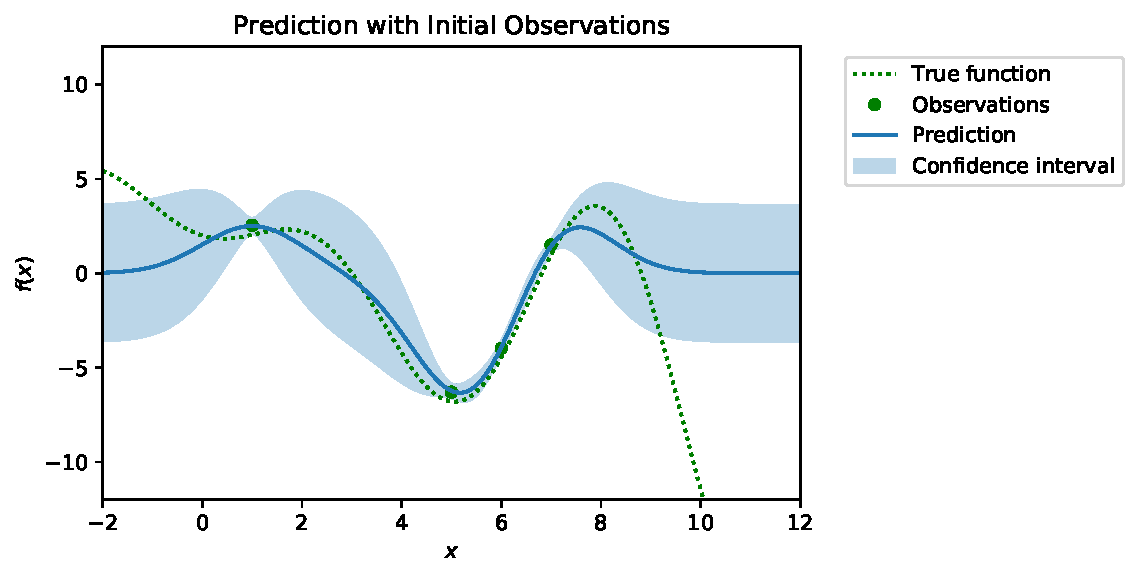
\includegraphics[scale=0.7]{plots/Prediction with Initial Observations.pdf}
%     \caption{Gaussian Process Regression Example. This plot shows the GPR prediction with confidence interval based on 4 initial observations. The confidence interval are shown in predicted mean $\pm$ 1.96 standard deviation.}
%     \label{fig: Gaussian Process Regression Example.}
% \end{figure}

The choice of covariance (kernel) function is critical for accurate predictions, since it controls smoothness and amplitude of the function we model.
To represent the RBS sequences and formulate the similarity between sequences, we use the \textit{weighted degree kernel with shift} (WDS) \cite{ratsch_rase_2005_wds} to specify the kernel function of $GP$.  
WDS is a type of a string kernel, which takes two sequences (strings) as inputs and outputs a scalar value which represents the similarities between the two sequences.  
WDS kernel does this by counting the matches of substrings of a certain length (i.e. kmers) that constitute the sequence.
The maximum substring length is specified by $\ell$. 
The WDS takes into account the positional information by counting substrings starting from different positions, where the start position is specified by $l$.
Additionally, the WDS kernel considers the shifting of substrings, with the maximum shift specified by $s$.
For example, for two core sequences \textit{ACCTGA} and \textit{CCTGAA}, there is a common part \textit{CCTGA} which is begins at the 2nd nucleotide in sequence 1 and at the 1st nucleotide in sequence 2, hence the calculated shift would be 1.

Let $\mathbb{I}$(A) is the indicator function, which equals 1 if $A$ is true and 0 otherwise. 
Then $\mathbb{I}(\mathbf{x}_{[l+s:l+s+d]} = \mathbf{x}_{[l:l+d]}^\prime)$ counts the matches of substrings of length $d$ between $\mathbf{x}$ starting from position $l+s$ and $\mathbf{x}^\prime$ starting from position $l$.
This is similarly done for $\mathbb{I}(\mathbf{x}_{[l:l+d]}= \mathbf{x}_{[l+s:l+s+d]}^\prime)$.
By having these two terms considering substrings of two sequences with starting positions differing by $s$ characters, the WDS can measure shifted positional information. 
When $s = 0$, the kernel function counts the matches with no shift between sequences. 
Let $\mathbf{x}, \mathbf{x}^\prime$ be two RBS sequences with length $L$, the WDS kernel is defined as
\begin{align}
        k_\ell^{WDS}(\mathbf{x}, \mathbf{x}^\prime) 
        %&= \sum_{d=1}^{\ell} \beta_d \sum_{l=1}^{L-d+1} \gamma_l \sum_{s = 0, s + l \leq L}^{S(l)} \delta_s
        %\left(k_d^{Spec}(\mathbf{x}_{[l+s:l+s+d]}, \mathbf{x}_{[l:l+d]}^\prime) + (k_d^{Spec}(\mathbf{x}_{[l:l+d]}, \mathbf{x}_{[l+s:l+s+d]}^\prime)\right)\\
        = \sum_{d=1}^{\ell} \beta_d \sum_{l=1}^{L-d+1} \gamma_l \sum_{s = 0, s + l \leq L}^{S(l)} \delta_s
        \left(\mathbb{I}(\mathbf{x}_{[l+s:l+s+d]} = \mathbf{x}_{[l:l+d]}^\prime) + (\mathbb{I}(\mathbf{x}_{[l:l+d]}= \mathbf{x}_{[l+s:l+s+d]}^\prime)\right),
\end{align}
where 
$\beta_d = \frac{2(\ell - d + 1)}{\ell(\ell+1)}, \delta_s = \frac{1}{2(s+1)}$, $\gamma_l$ is a weighting parameter over the position in the
sequence, where we choose to use a uniform weighting over the sequences, i.e. $\gamma_l = 1/L$. $S(l)$ determines the shift
range at position $l$. 

    
    
%  For recommendations, we consider the \textit{Upper Confidence Bound (UCB)} type algorithms. 
%  As one popular type of the bandit algorithms \cite{lattimore2018bandit}, the UCB type of algorithms are based on the \textit{optimism in the face of uncertainty},
 %provide various approaches to sequential design where an agent adaptively chooses one or more options among several actions based on certain policies. In our work we used the Upper Confidence Bound version of that algorithm, which is based on the \textit{optimism in the face of uncertainty}. The UCB algorithm, as the name suggests,
%  which basically select RBS sequences with the maximum upper confidence bound constructed by the sum of the predicted mean and $n$ standard deviation ($n > 0$), i.e. $\operatorname{argmax}_{\mathbf{x}_i \in \mathcal{D}} \left( \mu_t(\mathbf{x}_i) + \beta_t \sigma_t(\mathbf{x}_i)\right)$,
%     where $\beta_t$ is a hyperparameter balancing the exploitation and exploration, 
%     $\mu_t(\mathbf{x}_i), \sigma_t(\mathbf{x}_i)$ are the predicted mean and standard deviation at round $t$ for the sequence $\mathbf{x}_i$. 

\subsubsection{DESIGN: Batch UCB}

For recommendations of RBS sequences that should be experimentally labeled next, we have used the \textit{Upper Confidence Bound (UCB)} algorithm.
On one hand, we want to exploit the function in terms of the design space, that is to pinpoint sequences that are believed to have high labels (i.e. high predicted mean); 
on the other hand, we also want to explore the design space where we have little information and sequences have a chance to have high labels (i.e. high predicted SD).
The UCB algorithm provides such $\textit{exploitation-exploration balance}$ by balancing the predicted mean and SD.
More precisely, UCB algorithm selects RBS sequences with the maximum upper confidence bound at round $t$, i.e.
\begin{align}
\label{Eq: GPUCB}
    \operatorname{argmax}_{\mathbf{x}_i \in \mathcal{D}} \left( \mu_{t-1}(\mathbf{x}_i) + \beta_t \sigma_{t-1}(\mathbf{x}_i)\right),
\end{align}
where $\beta_t$ is a hyperparmeter balancing the exploitation and exploration, 
$\mu_t(\mathbf{x}_i), \sigma_t(\mathbf{x}_i)$ are the predicted mean and standard deviation (SD) at round $t$ for the sequence $\mathbf{x}_i$.
We call $\mu_{t-1}(\mathbf{x}_i) + \beta_t \sigma_{t-1}(\mathbf{x}_i)$ the \textit{UCB score} of sequence $\mathbf{x}_i$ at round $t$.

Since experimentally labelling sequences is time-consuming, it is unrealistic to recommend sequence sequentially (i.e. one-by-one) and then wait for the label to be tested and used to improve the model.
Instead, we can recommend RBS sequences in a batch of size $n$. 
One naive approach is to 
%train GP on sequences with known TIR labels and
recommend sequences in design space with top $n$ UCB scores, as shown in Figure \ref{fig:batch rec}(a) ($n = 2$).
However, this approach may end up recommending similar sequences in the same local maximum (e.g. $x = 2, x =2.5$ in this example). 
However, since we assume similar sequences would have similar labels (e.g. by knowing $x=2$ we can gain information of $x=2.5$ as well), we prefer to not waste time and money on labelling sequences with high similarities in the same batch.

% \begin{figure}[t]
% \centering
% \subfloat{\label{main:c}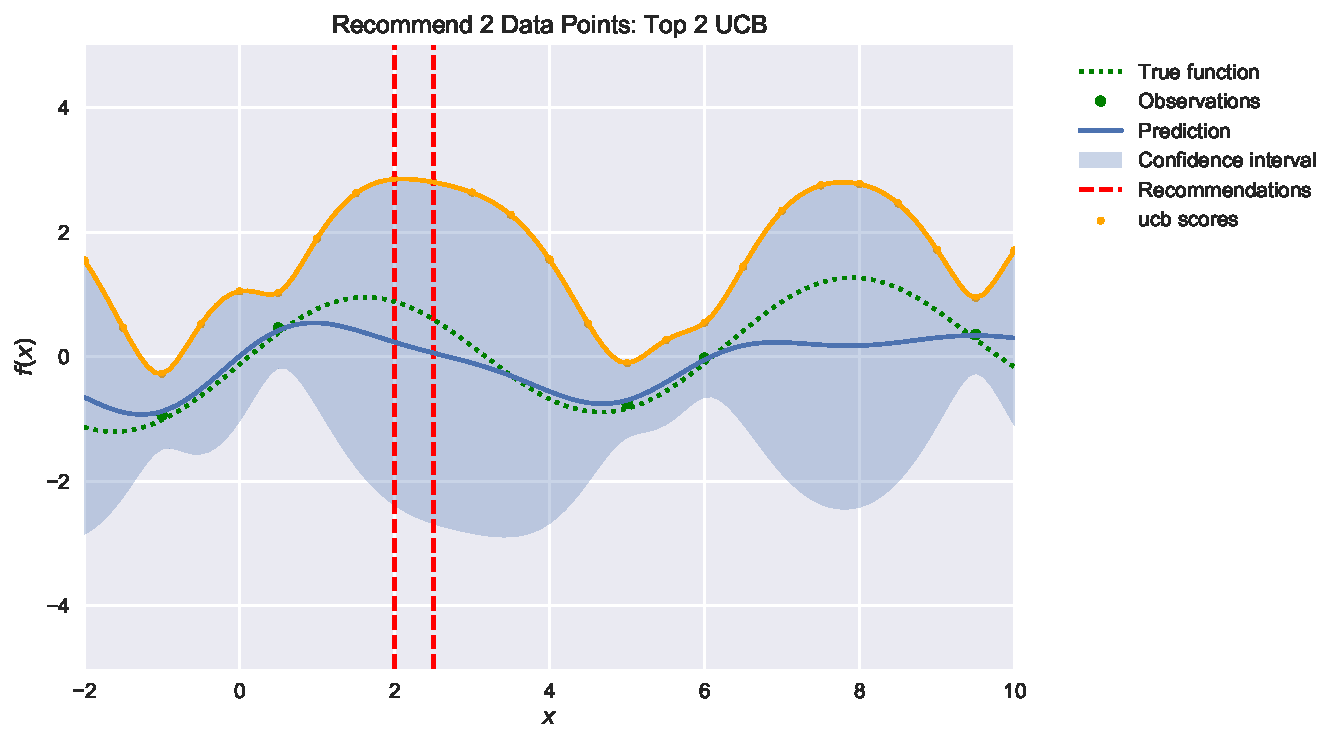
\includegraphics[scale=.4]{plots/Recommend_2_Data_Point_Top_2_UCB.pdf}}\par\medskip
% \begin{minipage}{.5\linewidth}
% \centering
% \subfloat{\label{main:a}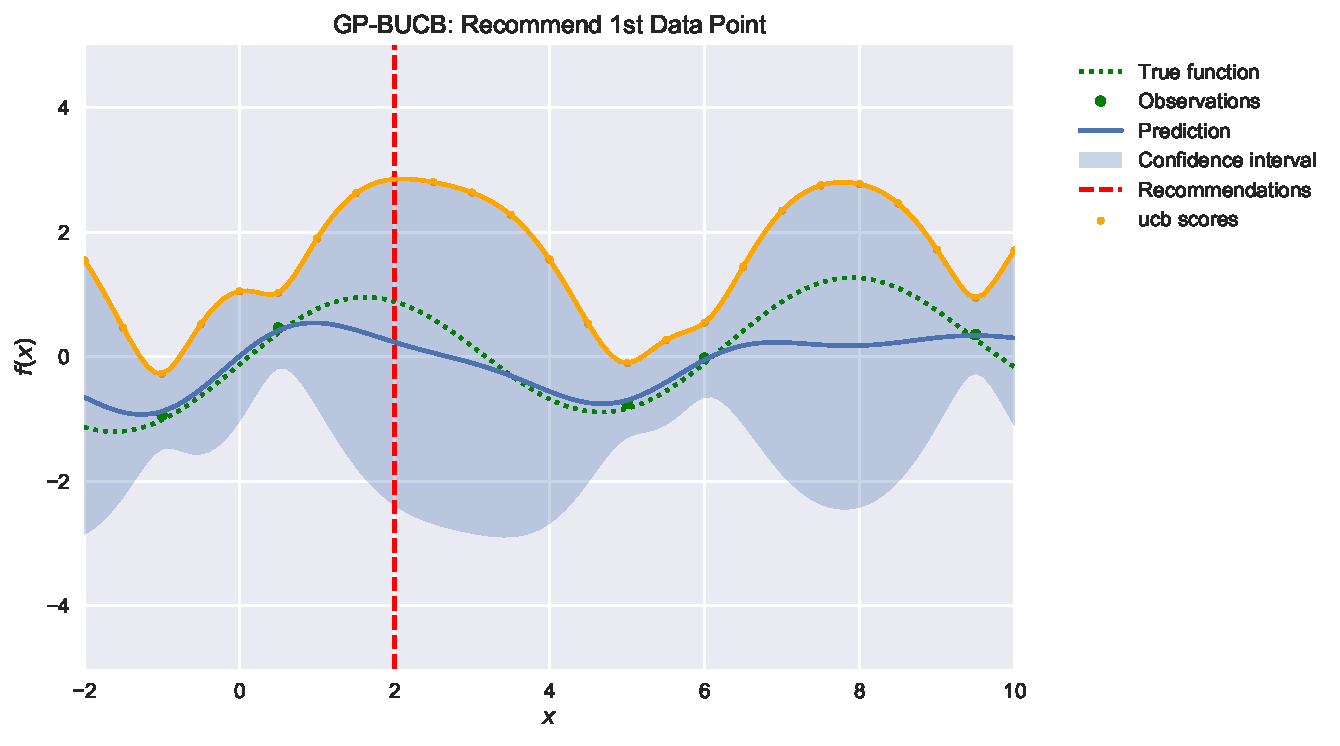
\includegraphics[scale=.4]{plots/GP-BUCB_Recommend_1st_Data_Point.pdf}}
% \end{minipage}%
% \begin{minipage}{.5\linewidth}
% \centering
% \subfloat{\label{main:b}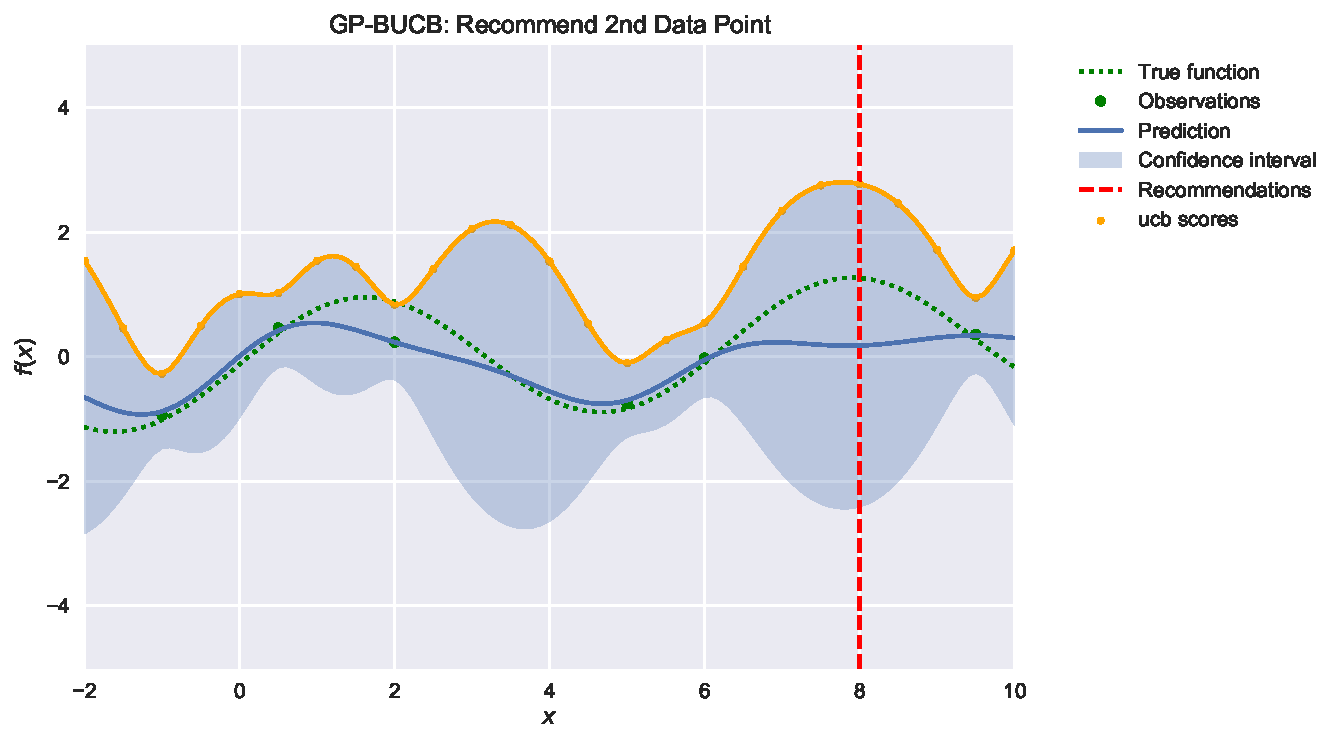
\includegraphics[scale=.4]{plots/GP-BUCB_Recommend_2nd_Data_Point.pdf}}
% \end{minipage}
% \caption{Batch Recommendation. We use the batch size of 2, with 5 initial observations. The design (recommendation) space is 24 uniformly distributed points in the range [-2,10], i.e. {-2, -1.5, -1, ..., 9.5, 10}.
% The confidence interval are shown with predicted mean of $\pm$ 1.96 standard deviation.
% (a) Top UCB recommendations. The recommendations are 2 data points with top UCB scores, constructed with GP predictions. 
% (b)(c) GP-BUCB recommendations. (b) shows the first recommended sequence, (c) shows the new predicted confidence interval and the second recommendation based on that.}
% \label{fig:batch rec}
% \end{figure}

\begin{figure}
    \centering
    \begin{subfigure}[b]{0.49\textwidth}
        \centering
        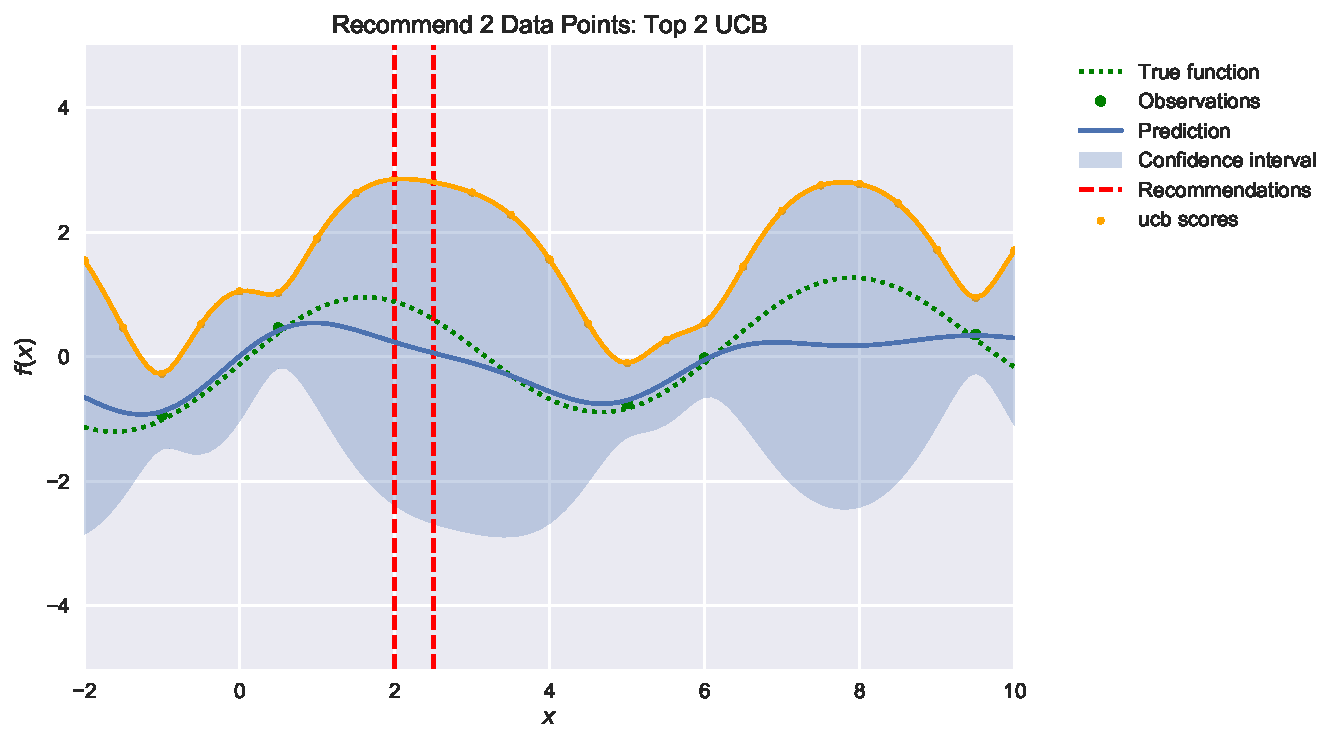
\includegraphics[scale=.4]{plots/Recommend_2_Data_Point_Top_2_UCB.pdf}
    \end{subfigure}
    \vskip\baselineskip
    \begin{subfigure}[b]{0.49\textwidth}
        \centering
        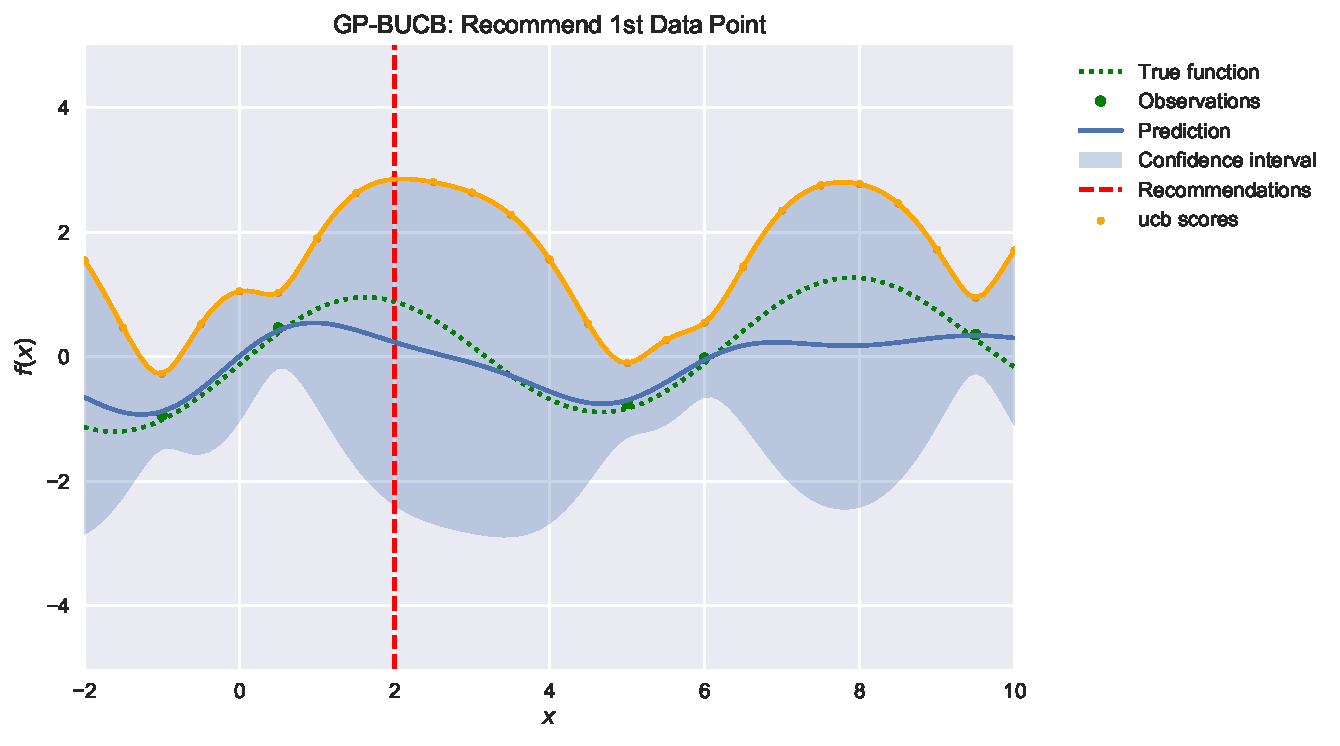
\includegraphics[scale=0.4]{plots/GP-BUCB_Recommend_1st_Data_Point.pdf}
    \end{subfigure}
    \hfill
    \begin{subfigure}[b]{0.49\textwidth}
        \centering
        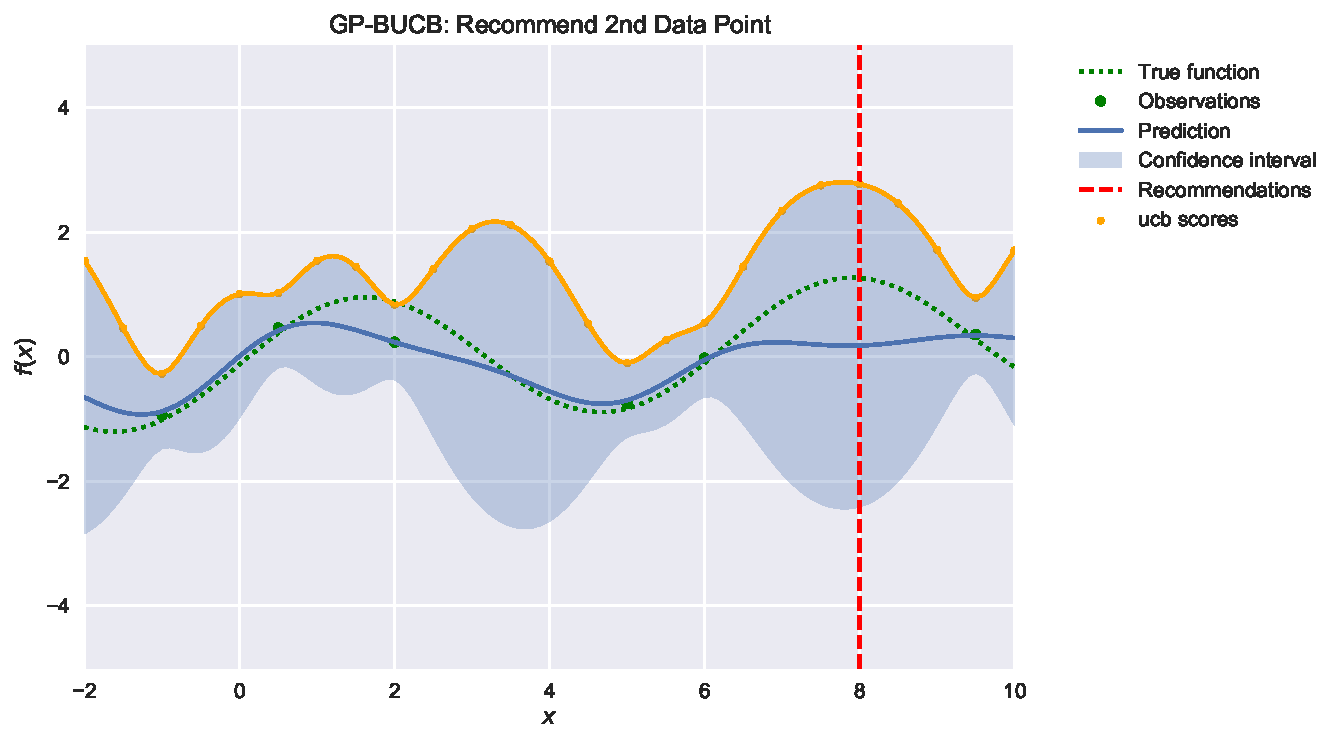
\includegraphics[scale=0.4]{plots/GP-BUCB_Recommend_2nd_Data_Point.pdf}
    \end{subfigure}
    \caption{Batch Recommendation. We use the batch size of 2, with 5 initial observations. The design (recommendation) space is 24 uniformly distributed points in the range [-2,10], i.e. {-2, -1.5, -1, ..., 9.5, 10}.
    The confidence interval are shown with predicted mean of $\pm$ 1.96 standard deviation.
    (a) Top UCB recommendations. The recommendations are 2 data points with top UCB scores, constructed with GP predictions. 
    (b)(c) GP-BUCB recommendations. (b) shows the first recommended sequence, (c) shows the new predicted confidence interval and the second recommendation based on that.}
    \label{fig:batch rec}
\end{figure}


A key property of Gaussian Process regression is that the predictive variance  depends only on observed points (i.e. features), but not on the labels of those observed points. 
% We illustrate this fact by comparing the prediction with the true function value of the new recommended point (Figure \ref{fig: Recommend 1 Data Point (New Observation)}) and the prediction with the predicted value of the new recommended point (Figure \ref{fig: Recommend 1 Data Point (Predicted Mean)}).
% As we can see, the predicted confidence interval is the same for the two plots. 
We can make use of this property to design batch upper confidence bound (BUCB) algorithm \cite{desautels2012parallelizing}.
That is, we can recommend sequences sequentially by updating the UCB score with the updated predicted SD with the the previously recommended points.
% Figure \ref{fig: Recommend 2 Data Points: GP-BUCB.} shows an example of batch UCB recommendation. 
% The plot shows the predicted mean and variance after observing 4 data points. 
First, GP-BUCB  recommends the data point with maximum UCB score based on the predictions over initial 5 observations as shown in Figure \ref{fig:batch rec}(b).  
Then we add the recommended data point ($x = 2$) into the training data set with the predicted mean of that point as label (note it is not the true label, i.e. observation), and update the predicted variance and then we finally update the UCB scores. We then recommend the second data point based on the new UCB scores.   
As we can see in Figure \ref{fig:batch rec}(c), since we assume we have observed $x = 2$, then the new predicted variance of the data points in design space around $x =2$  decreases, so instead of recommending a similar data point $x = 2.5$, we recommend the data point which is in a different maximum area with potentially high labels ($x = 8$).     
By using GP-BUCB, we can ensure that the sequences with high similarities will not be recommended in the same batch hence increasing the exploration efficiency. 
